\chapter{Confidentiality of Amounts in Grin}
\label{chap:grin-ub}

% *** SHORT DEFINITIONS ***
\newcommand{\amt}{\mathfrak{a}}
\newcommand{\rew}{\textit{reward}}
\newcommand{\fees}{\textit{fees}}

% \section{Introduction}
% no \IEEEPARstart
% Since the inception of Bitcoin, a wide range of crypotcurrencies came into existence post 2009 basing on different cryptographic primitives.
% The rise of new cryptocurrency models is inspired by the goal of acheiving privacy and anonymity guarantees along with scalability considerations.
% Monero was the first privacy-focused cryptocurrency which is based on the CryptoNote protocol \cite{Saberhagen2013}.
% However, Monero suffers the drawback of scalability implicitly because of the format of Ring Confidential Transactions \cite{Noether2016} it uses.
% With the ambition of establishing a full-fledged privacy coin, Grin \cite{GrinWebsite} was launched in January 2019. Making this ambition of Grin a reality
% is based on its implementation of Mimblewimble \cite{GrinDocOnGithub} protocol. Leveraging the homomorphic property of Pedersen commitments \cite{Pedersen91}, 
% Grin's cryptographic architecture allows draining off most data from the blockchain, offering significant scalability.  


MimbleWimble \cite{MimbleWimbleWhitePaper} is a scalable cryptocurrency design where coins are stored in Pedersen commitments \cite{Pedersen91}. 
The blinding factor of the Pedersen commitment which obscures the amount of coins also serves as the spending key. 
Like many other cryptocurrency designs, transactions in MimbleWimble are of two types: \textit{regular transactions} and \textit{coinbase transactions}. 
Regular transactions involve a transfer of coins from some input commitments already present on the blockchain to new output commitments. 
A combination of digital signatures and range proofs are used to prove that the total coins in the input commitments equals the total coins in the output commitments plus transaction fees, without revealing the amounts in the commitments \cite{GrinDocOnGithub}. 
Coinbase transactions reward miners for adding blocks to the blockchain. 
They only consist of output commitments and have no input commitments. 
The total amount of coins in the coinbase output commitments of a block is \textit{public}, being equal to the sum of the block subsidy and the transaction fees paid by the regular transactions in the block.

\blfootnote{Some sections of this chapter originally appeared in \cite{GrinUB1}.}
Every regular transaction output commitment can be traced back to a set of \textit{donor} coinbase output commitments with public amounts which could have possibly contributed to it. The key observation is that \textit{the amount of coins in a regular transaction output is bounded from above by the sum of the public amounts in its donor coinbase outputs minus the total transaction fees paid on the paths from these donor coinbase outputs to the regular transaction output}. While this observation is probably well-known in the MimbleWimble community, to the best of our knowledge there has been no effort to quantitatively compute such upper bounds for a MimbleWimble-based cryptocurrency. In this paper, we compute these upper bounds for the Grin implementation \cite{GrinWebsite} of MimbleWimble. Our method can be applied to the other implementations like Beam \cite{BeamWebsite}. We chose Grin because we were able to obtain its blockchain data from the administrator of the GrinExplorer site \cite{GrinExplorerWebsite}. Note that, unlike other cryptocurrencies, it is not possible for a new node in Grin to download all the historical blocks starting with the genesis block \cite{GrinForumReply}. This is a deliberate design choice as the MimbleWimble protocol does not require all the blocks to check the validity of the current blockchain state.
The network load on existing nodes in the Grin P2P network is reduced by not requiring them to send historical blocks to new nodes.\footnote{Beam does allow the download of all historical blocks from its P2P network, in addition to allowing the download of a compressed blockchain state like Grin.}

%Grin \cite{GrinWebsite} is a recently proposed cryptocurrency built using the MimbleWimble \cite{GrinDocOnGithub} protocol promising unlinkability under certain conditions as well as confidentiality of amounts.
%Leveraging the homomorphic property of Pedersen commitments \cite{Pedersen91}, Grin's cryptographic architecture allows draining off most data from the blockchain, offering significant scalability.
% It presents a scalable model of cryptocurrency coupled with privacy and anonymity guarantees. 
% In this work, we perform a first-hand analysis of the anonymity promises of outputs in Grin. 
% Each output in Grin is a Pedersen commitment hiding the amount it stores.
%Grin does not have any addresses as in Bitcoin \cite{Satoshi09} or Monero \cite{Noether2016}. Grin coins are stored in outputs which are Pedersen commitments.
%Pedersen commitments are perfectly hiding, i.e.\ they don't reveal anything about the amount they are committing to, even against a computationally unbounded adversary.
%In spite of this, it is interesting to assess if the underlying transaction structure in the design of a cryptocurrency system reveals anything about the amounts hidden in Pedersen commitments.

%Grin blocks contain transactions in an aggregated form. For each transaction in a block, the participants of that transaction have to publish a kernel excess which helps in verifying that no new money is being created.
%Since the transactions in a block are aggregated, it is not possible to link pairs of inputs and outputs from a particular transaction. 
%However, if the transaction pool itself contains very few transactions, it is possible to link inputs and outputs in an individual transaction. 
%In spite of the Dandelion protocol to ensure aggregation of transactions in the pooling phase itself, the low number of transactions on the Grin network allow such linking of inputs and outputs.
%For consistency with the original transaction structure of Grin, we choose to assume that transactions in each block are aggregated and linking inputs and outputs of individual transactions is not possible.
% We choose to assume that transactions in each block are aggregated and linking inputs and outputs is not possible for two reasons: 
% (i) To be consistent with the original transaction structure of Grin
% (ii) We wish to analyse blocks which are already present on the blockchain  

The first Grin block was mined on January 15, 2019. We used a snapshot of the blockchain from March 17, 2020 in our analysis which had 612,102 blocks. Grin has a block subsidy of 60 grins per block and a target inter-block time of one minute. Coinbase outputs cannot be spent until they receive 1440 confirmations which corresponds to 24 hours worth of blocks \cite{GrinCoinbaseMaturity}. For a regular transaction output (RTO) in a block at height $h$ (with genesis block having height 0), a trivial upper bound on the amount of coins in the output is $60 \times\max(0, h-1439)$ grins. This corresponds to the cumulative block subsidy in the blocks from height 0 to height $\max(0, h-1440)$. We define the \textit{flow upper bound} for an RTO to be the sum of the amounts in its donor coinbase outputs minus the total transaction fees paid in the paths from these donor coinbase outputs to the RTO (see Section \ref{scn:MainIdea} for an illustration). The effectiveness of the flow upper bound can be quantified using the \textit{flow ratio} of an RTO which is defined as
 \begin{align*}
  \text{Flow ratio of RTO} = \frac{\text{Flow upper bound of RTO}}{\text{Trivial upper bound of RTO}}.
\end{align*}
A value of flow ratio close to 1 implies that the flow upper bound does not reveal much information about the amount in the RTO. But a flow ratio value close to 0 implies that the flow upper bound is effective in constraining the amount in the RTO to a narrow range in the relative sense.

%The source of generation of new Grin coins is the constant reward earned by mining blocks. For each block mined, this reward along with transaction fees is deposited in the \textit{coinbase} output in that block.
%% For each block mined on the Grin blockchain, a reward of constant amount of grin coins is deposited in \textit{coinbase} output.
%Trivially so, the amount in the coinbase outputs is known. When such coinbase outputs are spent, the reward amounts are transferred to different \textit{transaction} outputs.
%We attempt to uncover how these known amounts from coinbase outputs flow to subsequent outputs appearing on the Grin blockchain.
%For example, the block at height $1449$ contains $1$ input, $2$ transaction outputs and $1$ coinbase output.
%Here, the input being spent is the coinbase output from block at height $2$ and the constant reward of $60$ grin flows into the $2$ transaction outputs.
%We thus get an upper bound on the amounts hidden in the transaction outputs. 
%We present an empirical graph-based analysis of the flow of grin coins from the blocks containing coinbase outputs to other blocks and establish upper bounds on the amount hidden in the transaction outputs in those blocks.
%The trivial upper bound on the amount stored in any output is the block height at which the output was generated times the constant reward.
%By studying the proximity of calculated upper bounds to the trivial bound, we aim to evaluate the confidentiality guarantees of amounts in Grin outputs.
% We observe that the ratio of calculated upper bounds and the trivial upper bound are close to unity for most of the transaction outputs in the blocks.
% This drives us to the conclusion that information leaked about the amounts in Grin outputs using such a graph-based analysis
% is negligible, strengthening the privacy argument of Grin. 


% Grin does not have any addresses as that of Bitcoin or Monero. Grin coins are stored in outputs which are Pedersen commitments.
% The only source of generation of new coins is the reward earned by mining blocks. For each block mined, this constant reward along with transaction fees is transferred to the \textit{coinbase} output in that block.
% Pedersen commitments are perfectly hiding, i.e.\ they don't reveal anything about the amount they are committing to, even against a computationally unbounded adversary.
% Although Grin outputs are Pedersen commitments, we exactly know the amount committed to in the coinbase outputs. 
% We attempt to uncover how these known amounts from coinbase outputs flow to subsequent outputs appearing on the Grin blockchain.
% Using the information available about the coinbase outputs, we present a mathematical formulation to analyse what could be conclusively said about the amounts in other outputs in the blockchain. 

% \textbf{Our Contribution}: 
\section{Our Contribution}
Our main contribution is an empirical analysis of the confidentiality of amounts in the Grin blockchain which takes the transaction graph into account. To enable efficient computation of the flow upper bound, we define a graph with vertex set equal to the union of the set of coinbase outputs and the set of blocks. Note that regular transaction inputs or outputs are not represented as vertices in this graph. The graph edges are defined to reflect all possible flows of coins between transaction inputs and outputs. Using this graph, we calculate the flow ratio as a function of the block height for the Grin blockchain (see Figure \ref{ratio-plot}). For the blocks in our snapshot, we find that the flow ratio is less than 0.5 for RTOs in 6.6\% of the blocks and more than 0.9 for 88\% of the blocks. As these statistics may be biased by early blocks mined during periods of low transaction activity, we consider the distribution of flow ratio for only unspent regular transaction outputs (URTOs) in our snapshot (see Figure \ref{utxo-plot}). We find that while 95\% of the 110,149 URTOs have a flow ratio greater than 0.9, about 0.8\% of them have a flow ratio less than 0.01. We conclude that while the flow upper bound does not violate the confidentiality of most of the URTOs, it can constrain the amounts in some URTOs to a narrow range.

%\textbf{Our Contribution}: We present a graph-based analysis of the Grin blockchain to give upper bounds on the amounts stored in the Grin outputs. 
%Our primary contribution is to examine the confidentiality claims of Grin with respect to the amounts in the outputs.
%To the best of our knowledge, our analysis is the first of its kind to answer the questions on privacy of Grin outputs.
%For an output in a block at height $h$, the trivial upper bound on the amount committed to is $h$ times the mining reward.
%We present a comparison of empirically computed upper bounds with trivial upper bounds for each output on the Grin blockchain.   
%The ratio of calculated and trivial upper bounds on the amounts in more than $87\%$ of the total transaction outputs on the Grin blockchain is greater than $0.9$.
%This implies that tracing the flow of coins from coinbase outputs to different outputs does not reveal any significant information about the amounts in those outputs. 
%This substantiates the confidentiality claim of amounts in Grin outputs.

\section{Related Work}
Inputs and outputs from disparate transactions are aggregated in a MimbleWimble block which hides the link between those involved in the same transaction. Ivan Bogatty \cite{Bogatty19} demonstrated a practical attack to uncover links between inputs and outputs in a Grin block by listening to transactions broadcast in the peer-to-peer network. We can obtain tighter flow upper bounds by incorporating such link information. Due to unavailability of such link information for historical blocks, we do not consider this information in the flow upper bound calculations described in this paper. So our results represent a conservative estimate of the upper bound and could be improved upon by incorporating links between inputs and outputs.

Apart from Bogatty's attack \cite{Bogatty19}, we are not aware of any other work addressing the privacy of MimbleWimble-based cryptocurrencies. To the best of our knowledge, our work is the first to address the confidentiality of amounts in MimbleWimble. Bogatty's attack is only concerned with linking inputs and outputs in a Grin block and does not consider privacy of amounts.
While Monero also has amounts hidden by Pedersen commitments, previous work addressing privacy in Monero by Kumar et al.~\cite{Kumar2017} and M\"oser et al.~\cite{Moser2018} has been primarily concerned with identifying the actual source address in the ring of addresses present in a Monero transaction. These papers do not address the privacy of amounts in Monero, which is an interesting direction for future work (our approach cannot be used directly due to the source address obfuscation in Monero).
%Linkability of sender and receiver in Grin transactions has long been a matter of discussion in the cryptocurrency community \cite{Loken17}.
%Ivan Bogatty \cite{Bogatty19} demonstrated a practical attack to uncover linkability in $96\%$ of the transactions in the transaction graph. 
%By listening to a lot of peer nodes, one can trace the origins of each transaction even if it is aggregated as per the Dandelion protocol.
%This is possible because by connecting to many peer nodes, it is highly probable that the parent node falls in the Dandelion path for any transaction.
%Using this approach, the question of who paid whom can be answered, but this talks nothing about the amounts being transferred. 
%% Bogatty states that no information about the amounts in the outputs can be recovered using this approach, only who paid whom in a Grin transaction can be traced.    
%Our work focuses on analysing the confidentiality of amounts in the outputs per block on the Grin blockchain.



\section{Overview of Grin}
\label{scn:GrinOverview}

%Grin is an implementation of the MimbleWimble protocol and thus it does not have any addresses.
Let $\mathbb{G}$ be the secp256k1 elliptic curve group of order $n$.
In Grin, coins are stored in Pedersen commitments of the form $C = kG + aH$ where $k, a \in \mathbb{F}_n$ are scalars and $G, H \in \mathbb{G}$ are the generators of $\mathbb{G}$ with an unknown discrete logarithm with respect to each other.
%Also, the discrete logarithm relation between $G$ and $H$ is assumed to be unknown. Grin uses the elliptic curve group secp256k1.
The quantity $a$ is the amount stored in $C$ and $k$ is a randomly chosen scalar known as the blinding factor. 
A Grin block consists of the following:
\begin{enumerate}
  \item[(i)] A block header from which a scalar $k_{\text{off}} \in \mathbb{F}_n$ called the \textit{kernel offset} can be derived. The other header fields are not relevant to our discussion.
  \item[(ii)] A list of $L$ input commitments $I_1, I_2,\ldots,I_L$. This list is empty for blocks without regular transactions. Each input commitment refers to an output commitment in a previous block.
  \item[(iii)] A list of $M$ output commitments $O_1, O_2,\ldots,O_M$ where $M \ge 1$. Each output commitment is tagged as either a coinbase output or a regular transaction output. Each output commitment is also accompanied by a range proof to prove that it commits to an amount in the range $\{0,1,2, \dots,2^{64}-1\}$.  
  \item[(iv)] A list of $N$ \textit{transaction kernels} each of which contains a fee amount $f_i \in \mathbb{F}_n$ and a curve point $X_i \in \mathbb{G}$ called the \textit{kernel excess}. Each kernel also contains a Schnorr signature proving that $X_i$ is of the form $x_iG$ for some $x_i \in \mathbb{F}_n$. Each transaction kernel is also tagged either as a coinbase kernel or a regular transaction kernel.
\end{enumerate}
% Each of these commitments refers to an output commitment in a previous block.An output is known as a \textit{coinbase} output if it is included by miners to store the mining reward and fees they earn
%during block mining. This transaction is known as \textit{coinbase} transaction.
%An output as a part of a regular transaction is known as \textit{transaction} output. 
%Each output is accompanied by a range proof to prove that it commits to an amount in the range $\{0,1,2, \dots,2^{64}-1\}$.  
%A Grin transaction consists of the following entities:
%\begin{enumerate}
%  \item[(i)] A vector of inputs serving as the sources of coins in the transaction. Each input is essentially an unspent output from some previous block.
%  \item[(ii)] A vector of outputs representing the destinations of coins in the transaction.
%  \item[(iii)] A vector of transaction kernels which are used in verification of transaction validity.
%\end{enumerate}
%A kernel is either a coinbase or a plain kernel according to the type of transaction.
%% A plain kernel is called as \textit{height-locked} kernel if the underlying transaction restricts its inclusion until a block at a specified height is mined.
%Each kernel contains the transaction fee and a \textit{kernel excess} which is a point on the curve of the form $xG$ where $x \in \mathbb{F}_n$.
%The kernel excess is accompanied by a Schnorr signature proving that it is of the form $xG$.
%% Transaction fee is included as a part of the kernel.
%
%A Grin block is characterized by a unique field called \textit{hash} which is SHA256 hash of its contents.
%% Each block contains the details of the Proof-of-Work used for mining.
%The inputs and outputs in a block are aggregated and we cannot distinguish between inputs and outputs of individual transactions.
%However, the total number of transactions in a block is equal to the number of kernels in that block.
%Suppose a block contains $L$ inputs $I_1, I_2, \dots, I_L$, $M$ outputs $O_1,O_2, \dots, O_M$
%and $N$ kernel excesses $X_1, X_2 \dots, X_N$ with individual fees $f_1, f_2 \dots, f_N$.
Let $\mathcal{I}_{\text{cb}} \subset \{1,2,\ldots,M\}$ be the set of indices corresponding to coinbase outputs and $\mathcal{I}_{\text{cb}}^c$ be the set of the remaining indices corresponding to RTOs. Let $\mathcal{I}_{\text{ck}} \subset \{1,2,\ldots,N\}$ be the set of indices corresponding to coinbase kernels and $\mathcal{I}_{\text{ck}}^c$ be the set of indices corresponding to regular transaction kernels. A valid block has to satisfy the following equations.
\begin{align}
  \sum_{i \in \mathcal{I}_{\text{cb}}} O_i - \left(\sum_{i=1}^{N}f_i\right)H - r H & = \sum_{i \in \mathcal{I}_{\text{ck}}} X_i,\\
  \sum_{i \in \mathcal{I}_{\text{cb}}^c} O_i + \left(\sum_{i=1}^{N}f_i\right)H - \sum_{i=1}^{L} I_i & = \sum_{i \in \mathcal{I}_{\text{ck}}^c} X_i + k_{\textnormal{off}}G.
  %\sum_{i=1}^{L} O_i + \left(\sum_{i=1}^{N}f_i\right)H - \sum_{i=1}^{M} I_i = \sum_{i=1}^{M} X_i + k_{\textnormal{off}}G
  \label{eqn:BlockValidity}
\end{align}
Here $r = 60\times 10^9$ is the block subsidy in nanogrin units.
As the right hand sides of both equations are commitments to the zero amount, the binding property of Pedersen commitments and the range proofs imply that
\begin{enumerate}
  \item[(i)] the total amount in the coinbase outputs of a block is $r + \sum_{i=1}^{N} f_i$ and
  \item [(ii)] the sum of the input amounts is equal to the sum of the transaction fees and RTO amounts.
\end{enumerate}
% The sum of coefficients of $H$ is zero in the above equation ensuring that no new coins are created.
%To see why (\ref{eqn:BlockValidity}) is enough to ensure validity of transactions, let
%$O_i = k_i^{\textnormal{out}}G + v_i^{\textnormal{out}}H$,
%$I_i = k_i^{\textnormal{in}}G + v_i^{\textnormal{in}}H$ and $X_i = x_iG$. Equation (\ref{eqn:BlockValidity}) holds only if the following hold
%\begin{align}
%  \sum_{i=1}^{M} v_i^{\textnormal{in}} &= \sum_{i=1}^{L} v_i^{\textnormal{out}} + \sum_{i=1}^{N}f_i \label{eqn:AmountEq} \\
%  \sum_{i=1}^{L} k_i^{\textnormal{out}} - \sum_{i=1}^{M} k_i^{\textnormal{in}} &= \sum_{i=1}^{N}x_i + k_{\textnormal{off}} \label{eqn:blindingFEq}
%\end{align}
%Equation (\ref{eqn:AmountEq}) implies that no new money was created and (\ref{eqn:blindingFEq}) implies that the coefficients of $G$ balance out.
%The reason for including $k_{\textnormal{off}}$ is to hide the relationship between the inputs and outputs in a block.
%If there were no kernel offset in a transaction, an adversary could attempt to deconstruct the individual transactions by trying combinations of inputs, outputs and kernels satisfying the transaction validity equation.
%
%A Grin block looks like a single transaction consisting of the aggregated inputs and outputs.
%If any output appears as an input in the same block, both of them are removed as they are not required for the block validation.
%Similarly, once an output is spent, it can be removed from the blockchain. 
%This process is known as \textit{cut-through} which improves scalability of Grin. 


\section{Illustration of Flow Upper Bound Calculation}
\label{scn:MainIdea}
In this section, we illustrate the flow upper bound calculation with an example.
Consider blocks at heights $h_1$, $h_2$, and $h_3$ on the Grin blockchain as shown in Figure \ref{block_sample}.
%For notational simplicity, we will refer to the block at height $h_1$ as block $h_1$ and so on.
% Each block has a coinbase output denoted by $O_1$.
Let the total fees for the block at height $h_i$ be $f^{\text{tot}}_i$.
The block reward in block $h_i$ is then $r_i = r + f^{\text{tot}}_i$ where $r=60$ grins is the block subsidy.
% The arrows denote the flow of coins.
An inter-block arrow from an output $O_l^{h_i}$ to an input $I_{j}^{h_{i+1}}$ denotes that the input is spending the output.
An intra-block arrow from an input $I_j^{h_i}$ to an output $O_l^{h_i}$ indicates that the input could be contributing coins to the output; however such an arrow does not indicate that the input is definitely contributing to the output. In the absence of linkability information, we assume any input in a block can contribute to any RTO in the same block.


Let $\mathfrak{a}(C)$ be the amount hidden in a commitment $C$.
We will assume that the first output $O_1^{h_i}$ is the only coinbase output in all three blocks. Then $\mathfrak{a}(O_1^{h_i}) = r_i$ for $i=1,2,3$.
The coinbase output $O_1^{h_1}$ is spent in block $h_2$ via the input $I_1^{h_2}$. So we have $I_1^{h_2} = O_1^{h_1} \implies \mathfrak{a}(I_1^{h_2}) = r_1$. The coinbase output $O_1^{h_2}$ and regular transaction output $O_3^{h_2}$ are spent in block $h_3$ via the inputs $I_1^{h_3}$ and $I_2^{h_3}$ respectively.
So we have $\ I_1^{h_3} = O_1^{h_2}$ and $I_2^{h_3} = O_3^{h_2}$ which implies $\mathfrak{a}(I_1^{h_3}) = r_2$ and $\mathfrak{a}(I_2^{h_3}) = \mathfrak{a}(O_3^{h_2})$.

\begin{figure}[!t]
  \centering
  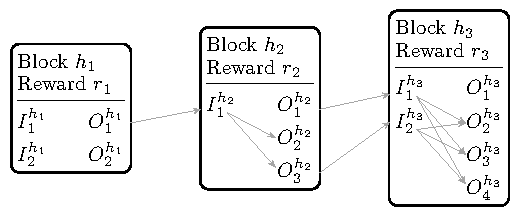
\includegraphics[width=0.65\textwidth]{Figures/grin_blocks1.pdf}
  \caption{llustration of flow upper bound calculation for blocks at height $h_1, h_2, h_3$.}
  \label{block_sample}
\end{figure}

%Similarly, coinbase output $O_1^{h_2}$ is spent in block $h_3$.
%Trivially, the amounts stored in coinbase outputs $O_1^{h_i}$ is $r_i$ for $i\in \{1,2,3\}$. 
% Outputs appearing as a part of transactions in a block are called as \textit{transaction} outputs.
%What is more interesting is to discover what the amounts in transaction outputs in a block could be. 
%Let us concentrate on the coinbase output $O_1^{h_1}$ in block $h_1$.
%When it is spent in block $h_2$, the reward $r_1$ \textit{flows} into the transaction outputs $O_2^{h_2}$ and $O_3^{h_2}$. 
% Now, when output $O_3$ from block $h_2$ appears as an input $I_2$ in block $h_3$, the coins flow to the transaction outputs $O_2, O_3, O_4$ in block $h_3$.
% Similar flow of coins occurs from coinbase output $O_1$ in block $h_2$.
%Thus, we have
The consequence of equation (\ref{eqn:BlockValidity}) in block $h_2$ is 
\begin{align}
  \amt(O_2^{h_2}) + \amt(O_3^{h_2}) = r_1 - f^{\text{tot}}_2.
\end{align}
While the sum of the amounts in $O_2^{h_2}$ and $O_3^{h_2}$ is known, the allocation of the sum to each output is hidden. As the sum represents an upper bound on the individual amounts in each of the outputs, we have
\begin{align}
  \amt(O_l^{h_2})\le r_1 - f^{\text{tot}}_2 \ \ \ \text{ for } l = 2,3.
  \label{eqn:UB1}
\end{align}
The term on the right hand side is the flow upper bound for the RTOs in block $h_2$. The set of donor coinbase outputs for $O_2^{h_2}, O_3^{h_2}$ contains only $O_1^{h_1}$ which contributes $r_1$ to the upper bound. The $f_2^{\text{tot}}$ term corresponds to the total fees paid on the path from the donor coinbase output $O_1^{h_1}$ to the RTOs $O_2^{h_2}, O_3^{h_2}$. In general, the flow upper bound is the same for all the RTOs in the same block.

The consequence of equation (\ref{eqn:BlockValidity}) in block $h_3$ is 
\begin{align*}
  & \amt(O_2^{h_3}) + \amt(O_3^{h_3}) + \amt(O_4^{h_3}) \nonumber \\
  & = \amt(I_1^{h_3}) + \amt(I_2^{h_3}) - f^{\text{tot}}_3 \nonumber \\
  & = \amt(O_1^{h_2}) + \amt(O_3^{h_2}) - f^{\text{tot}}_3 \nonumber \\
  & = r_2 + \amt(O_3^{h_2}) - f^{\text{tot}}_3 \nonumber \\
  &  \le r_2 + r_1 - f^{\text{tot}}_2 - f^{\text{tot}}_3,
\end{align*}
%\begin{align*}
%  & \amt(O_2^{h_3}) + \amt(O_3^{h_3}) + \amt(O_4^{h_3})= \amt(I_1^{h_3}) + \amt(I_2^{h_3}) - f^{\text{tot}}_3 \nonumber \\
%  \implies & \amt(O_2^{h_3}) + \amt(O_3^{h_3}) + \amt(O_4^{h_3})= \amt(O_1^{h_2}) + \amt(O_3^{h_2}) - f^{\text{tot}}_3 \nonumber \\
%  \implies & \amt(O_2^{h_3}) + \amt(O_3^{h_3}) + \amt(O_4^{h_3})= r_2 + \amt(O_3^{h_2}) - f^{\text{tot}}_3 \nonumber \\
%  \implies & \amt(O_2^{h_3}) + \amt(O_3^{h_3}) + \amt(O_4^{h_3}) \le r_2 + r_1 - f^{\text{tot}}_2 - f^{\text{tot}}_3,
%\end{align*}
where the last inequality follows from equation (\ref{eqn:UB1}). Once again the upper bound on the sum of the amounts in the RTOs, yields the flow upper bound on the individual amounts given by
\begin{align}
  \amt(O_l^{h_3})  \le r_2 + r_1 - f^{\text{tot}}_2 - f^{\text{tot}}_3 \ \ \ \text{ for } l =2,3,4.
  \label{eqn:UB2}
\end{align}
The $r_2 + r_1$ term in the flow upper bound is due to the donor coinbase outputs $O_1^{h_1}, O_2^{h_2}$ and the $f^{\text{tot}}_2 + f^{\text{tot}}_3$ term corresponds to the total fees paid on the paths from these donor coinbase outputs to the RTOs in block $h_3$.
% \[\amt(O_2) + \amt(O_3) = r_1 - f^{\text{tot}}_2 \textnormal{ and}\]
% \[\emph{max}\{\amt(O_2), \amt(O_3)\} \le r_1 - f^{\text{tot}}_2 .\]
%Note that the fees $f^{\text{tot}}_2$ of block $h_2$ is subtracted since it is deposited in the coinbase output of block $h_2$. Thus, we have 
%\begin{equation}
%  \amt(O_j^{h_2}) \le r_1 - f^{\text{tot}}_2 \textnormal{ for } j \in \{2,3\}.
%  \label{eqn:UB1}
%\end{equation}
%Substituting $r_1 = r + f^{\text{tot}}_1$ in (\ref{eqn:UB1}), we get
%\begin{equation}
%  \amt(O_j^{h_2}) \le r + f^{\text{tot}}_1 - f^{\text{tot}}_2 \textnormal{ for } j \in \{2,3\}.
%  \label{eqn:UB2}
%\end{equation}
%Further, when $O_1^{h_2}$ and $O_3^{h_2}$ are spent in block $h_3$ as inputs $I_1^{h_3} \textnormal{ and } I_2^{h_3}$ respectively, the total amount spent is 
%\begin{equation*}
%  \amt(I_1^{h_3}) + \amt(I_2^{h_3}) \le (r_1 - f^{\text{tot}}_2) + r_2.
%\end{equation*}
%Thus, the total amount in transaction outputs in block $h_3$ is 
%\begin{gather*}
%  \amt(O_2^{h_3}) + \amt(O_3^{h_3}) + \amt(O_4^{h_3}) \le ((r_1 - f^{\text{tot}}_2) + r_2) - f^{\text{tot}}_3 \\
%  \intertext{Since the amounts in outputs is non-negative, the upper bound on the maximum amount in these outputs can be expressed as}
%  \therefore \emph{max}\{\amt(O_2^{h_3}), \amt(O_3^{h_3}), \amt(O_4^{h_3})\} \le ((r_1 - f^{\text{tot}}_2) + r_2) - f^{\text{tot}}_3 .
%\end{gather*}
%% \[\amt(O_2) + \amt(O_3) + \amt(O_4) = ((r_1 - f^{\text{tot}}_2) + r_2) - f^{\text{tot}}_3 \textnormal{ and}\]
%% \[\emph{max}\{\amt(O_2), \amt(O_3), \amt(O_4)\} \le ((r_1 - f^{\text{tot}}_2) + r_2) - f^{\text{tot}}_3 .\]
%Hence, the upper bound on the amount stored in transaction outputs in block $h_3$ can be expressed as 
%\begin{equation}
%  \amt(O_j^{h_3}) \le ((r_1 - f^{\text{tot}}_2) + r_2) - f^{\text{tot}}_3 \textnormal{ for } j \in \{2,3,4\}.
%  \label{eqn:UB3}
%\end{equation}
%Substituting $r_i = r + f^{\text{tot}}_i$ for $i=1,2$ in \ref{eqn:UB3}, we get 
%\begin{equation}
%  \amt(O_j^{h_3}) \le (2r + f^{\text{tot}}_1) - f^{\text{tot}}_3 \textnormal{ for } j \in \{2,3,4\}.
%  \label{eqn:UB4}
%\end{equation}
%Equations (\ref{eqn:UB2}), (\ref{eqn:UB4}) show that the upper bound on transaction outputs in a block depends on the number of \textit{donor} coinbase outputs from previous blocks in the blockchain.
%We formalise the notion of \textit{donor} coinbase outputs in Section \ref{subscn:ComputingUB}.
% Here, for transaction outputs in block $h_3$, the donor coinbase outputs are from blocks $h_1$ and $h_2$.
% Further, we can give a more compact upper bound by subtracting the fees from blocks which are not the immediate predecessors of the block in consideration.  

%Therefore, the upper bound on the amounts in the outputs in a particular block depends only on the amount of flow of coins from previous blocks in the blockchain.
%Consequently, the upper bounds on all the transaction outputs in a block are the same.
%We generalise this idea to estimate the upper bounds on the transaction outputs in blocks appearing on the Grin Blockchain using graph-based analysis.


\section{The Flow Graph}
\label{scn:FlowGraph}
% The upper bound on the amounts in the outputs in a particular block depends only on the amount of flow of coins from previous blocks in the blockchain.
% Consequently, the upper bounds on all the transaction outputs in a block are the same.
%Since the upper bound on the amounts in transaction outputs in a block is same, we need to estimate the flow of coins flowing into the blocks.
%% rather than actual outputs.
%More precisely, to calculate the upper bound in a block, we need to know the source of the inputs spent in that block. 
%% Suppose there are $p$ inputs in block $h_0$. Let the sources of these inputs be the blocks $h_{-1}^{(1)}, h_{-1}^{(2)}, \dots, h_{-1}^{(p)}$ and so on.  
%% Note that the $(-1)$ in the subscript denotes the input history at step $1$. 
%If a particular input was a coinbase output in a previous block where it was generated, we exactly know the amount carried by this input.
%If an input was a transaction output in a previous block, we need to further trace the source of coins flowing into that previous block.
%% Suppose such an input was generated in block $h_{-1}^{(k)} \textnormal{ for some } k \in \{1,2, \dots, p\}$. We again find the sources of inputs in the block $h_{-1}^{(k)}$ as blocks 
%% $h_{-2}^{(k,1)}, h_{-2}^{(k,2)}, \dots, h_{-2}^{(k,p_k)}$, where $p_k$ is the number of inputs in the block $h_{-1}^{(k)}$.
%We keep repeating this process until we find the coinbase output in the path traced for each of the inputs in the concerned block.
%The total upper bound then becomes the cumulative rewards each terminal coinbase outputs possesses. 

To automate the calculation of flow upper bounds, we construct a directed graph $G = (V, E)$ from the information available on the Grin blockchain, which we call the \textit{flow graph}. In the Grin blockchain snapshot we considered, every block had exactly one coinbase output even though this is not mandatory.\footnote{\url{https://github.com/mimblewimble/grin/issues/689}} We assume that this condition holds in our discussion below. 
%Here, $V, E$ is the set of all vertices and edges respectively.

Let $V_{\text{bl}}$ be the set of blocks in the blockchain and let $V_{\text{cb}}$ be the set of all coinbase outputs. %So we could uniquely identify a coinbase output by the height of its block.
%Each block $h \in V_{\text{bl}}$ contains a single coinbase output $c_h$.
% \[ N_{cb} \coloneqq \bigcup\limits_{h \in N_b} c_h \]
% as the set of all coinbase outputs. 
The set of vertices is defined as $V = V_{\text{bl}} \cup V_{\text{cb}}$. 
The set of directed edges $E$ will capture two types of flows of coins.
\begin{enumerate}
  \item[(i)] For $c \in V_{\text{cb}}$ and $b \in V_{\text{bl}}$, the directed edge $(c, b)$ belongs to the edge set $E$ if the coinbase output $c$ is spent by a regular transaction input in block $b$.
  \item[(ii)] For $b_1, b_2 \in V_{\text{bl}}$, the directed edge $(b_1, b_2)$ belongs to the edge set $E$ if \textit{at least} one regular transaction output in block $b_1$ is spent by a regular transaction input in block $b_2$.\footnote{Note that output being spent in block $b_1$ has to be an RTO and not a coinbase transaction output. The flow of coins out of coinbase outputs is captured by the previous type of edge. Also note that there can exist at most one edge between two blocks $b_1$ and $b_2$ as the edge existence condition requires only that at least one RTO in block $b_1$ be spent in block $b_2$.}
\end{enumerate}
The edge set $E$ has no other edges.
Note that the intra-block flow of coins from inputs to outputs in the same block has not been explicitly represented in the flow graph. This is because we are not taking linkability information about inputs and outputs into account.
For block $b \in V_{\text{bl}}$, Algorithm \ref{algo:subG} generates the subgraph $G_s^{(b)} = (V_s^{(b)}, E_s^{(b)}), \ V_s^{(b)} \subset V_{\text{bl}}, \ E_s^{(b)} \subset E$ and computes the set $R^{(b)} \subset V_{\text{cb}}$ of donor coinbase vertices.
Let \texttt{pred}($b$) denote the set of predecessors to node $b$.
\begin{algorithm}[h]
	\caption{Create subgraph for node $b \in V_{\text{bl}}$} 
 \begin{algorithmic}[1]
   \Procedure{\textnormal{\texttt{subG}}}{$b$}
   \For {$p \textnormal{ in } \texttt{pred}(b)$}
     \State $V_s^{(b)} \leftarrow V_s^{(b)} \cup \{p\}, \ E_s^{(b)} \leftarrow E_s^{(b)} \cup \{(p, b)\} $ \hfill{\footnotesize \textit{// Predecessors added to subgraph}}
     \If {$p \in V_{\text{cb}} \textnormal{ and } p \notin R^{(b)}$} \hfill{\footnotesize \textit{// Stop if coinbase node is found}}
       \State $R^{(b)} \leftarrow R^{(b)} \cup \{p\}$
     \Else \hfill{\footnotesize \textit{// Else continue recursively}}
     \State \texttt{subG}($p$)
     \EndIf
   \EndFor
   \EndProcedure
 \end{algorithmic} 
 \label{algo:subG}
\end{algorithm}

\begin{definition}
  A coinbase output vertex $c$ in $G$ is called a donor of a block $b$ if there is a directed path from $c$ to $b$ in $G$. A donor of a block $b$ is also referred to as the donor of the regular transaction outputs in the block $b$.
\end{definition}
For example, Figure \ref{subgraph-eg} shows the subgraph generated by the donor coinbase outputs of the block at height 1499 and the blocks which lie on paths from these coinbase outputs to it. 
The square vertices represent blocks and the circular vertices represent coinbase outputs labelled with the block height in which they were generated. Edges denote the flow of coins.
Block 1499 has 7 donors at block heights 5, 7, 9, 16, 18, 33, and 38. The flow upper bound for the RTOs in block 1499 is equal to the sum of the block rewards of these 7 coinbase outputs minus the transaction fees paid in the 9 blocks which lie on the paths from the 7 donors to 1499 (inclusive of 1499).
\begin{figure}[!t]
  \centering
  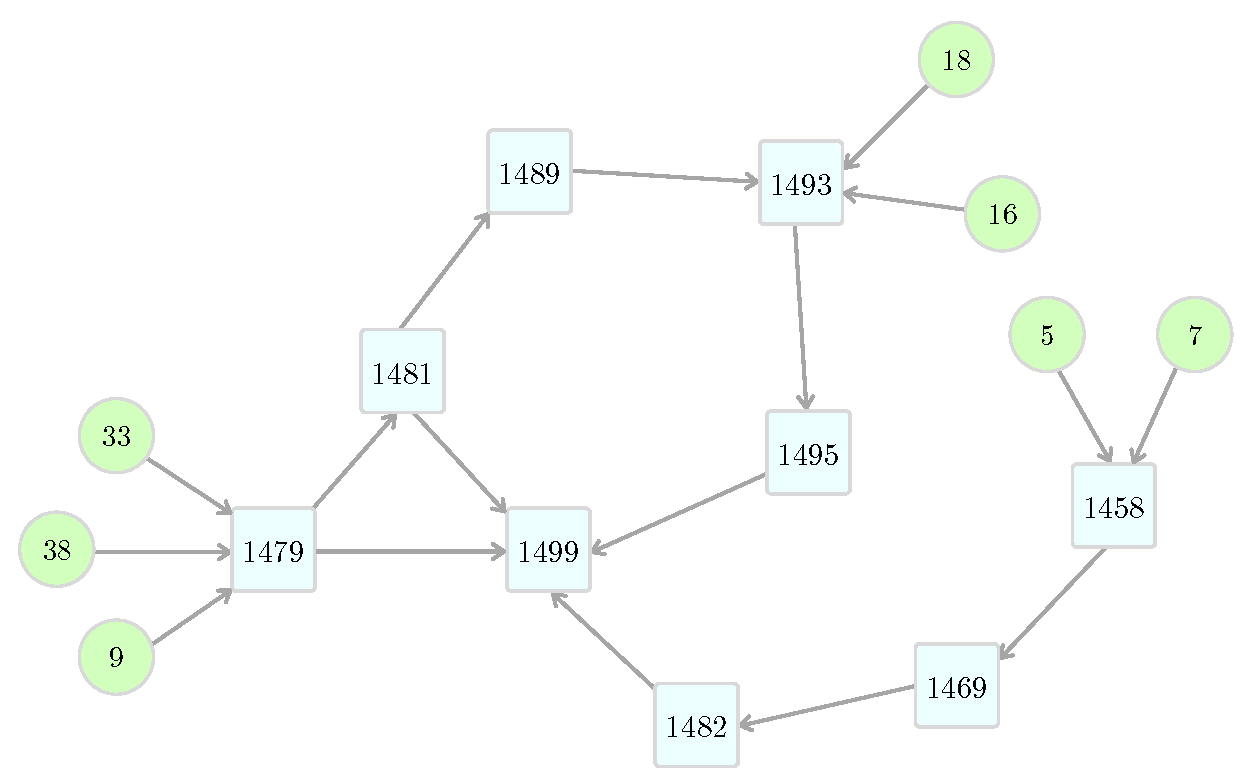
\includegraphics[width=0.9\textwidth]{Figures/subgraph1499.pdf}
  \caption{Subgraph generated for block at height $1499$.}
  \label{subgraph-eg}
\end{figure}


\begin{figure*}[t]
  \centering
  \captionsetup{justification=centering}
  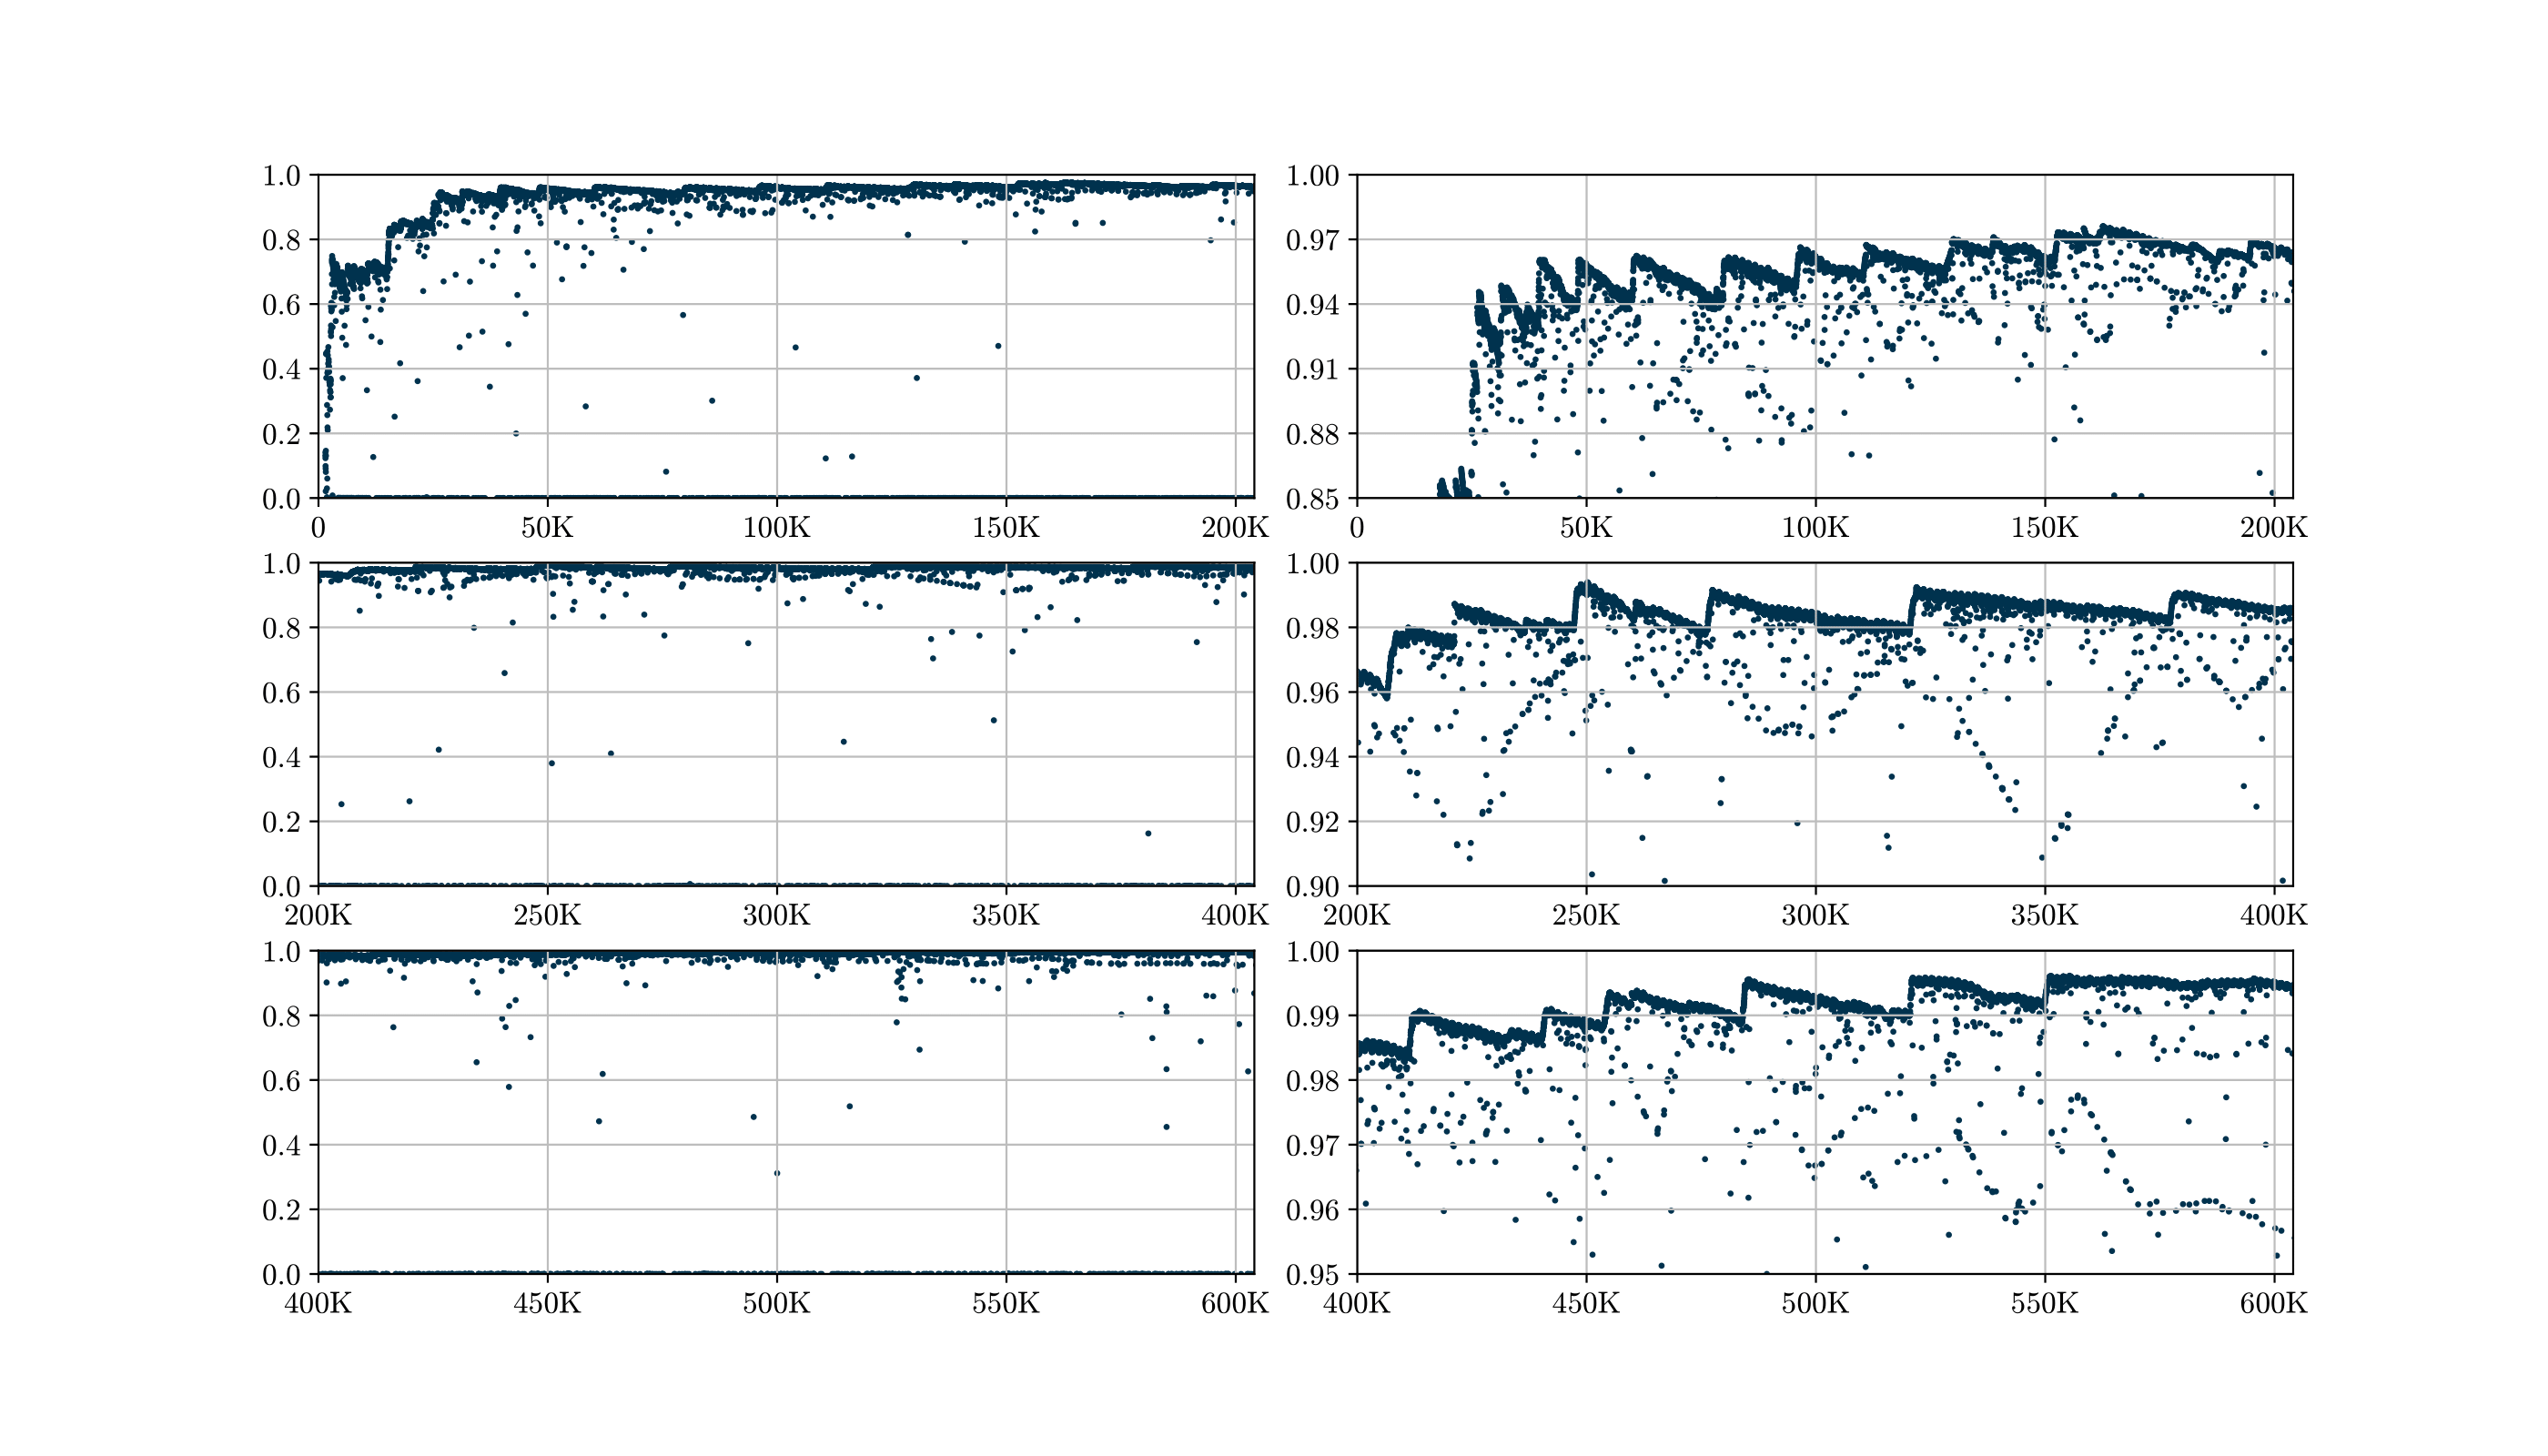
\includegraphics[width=\textwidth, trim={10cm 6cm 9cm 5cm},clip]{Figures/ratio_compact1-1.png}
  \vspace{-10pt}
  \caption{Plot of flow ratio vs block height. Plot of flow ratio close to 1 shown magnified on right.}
  \label{ratio-plot}
\end{figure*}
Let $V_{\text{cb}}^{(h)}$ be the set of donor coinbase outputs of the block at height $h$. Let $V_{\text{bl}}^{(h)}$ be the set of blocks which lie on a directed path in the flow graph $G$ from any vertex in $V_{\text{cb}}^{(h)}$ to the block at height $h$. The block at height $h$ is also included in $V_{\text{bl}}^{(h)}$.
For a coinbase output vertex $c \in V_{\text{cb}}$, let $\rew(c)$ denote the block reward (subsidy plus fees) of the block in which $c$ appeared.
For a block vertex $b \in V_{\text{bl}}$, let $\fees(b)$ denote the total transaction fees paid by all the regular transactions in block $b$.
For a regular transaction output $O$ in a block at height $h$, the flow upper bound is given by
\begin{align}
  \amt(O) \le \sum_{c \in V_{\text{cb}}^{(h)}} \rew(c) - \sum_{b \in V_{\text{bl}}^{(h)}} \fees(b).
  \label{eqn:FLUB}
\end{align}
The correctness of this upper bound can be argued as follows. It is clear that
\begin{align}
\amt(O) \le \sum_{c \in V_{\text{cb}}^{(h)}} \rew(c)
\end{align}
as the total coins in $O$ cannot exceed the sum of all possible sources of coins for block $h$. Let $f_{\text{tot}}^{(h)} = \sum_{b \in V_{\text{bl}}^{(h)}} \fees(b)$. We claim that the fees in $f_{\text{tot}}^{(h)}$ must be paid \textit{only} from the coins minted in coinbase outputs belonging to $V_{\text{cb}}^{(h)}$. If our claim is true, $f_{\text{tot}}^{(h)}$ must be deducted from the upper bound as these fees are paid before the coins reach the output $O$. To verify our claim, suppose coins minted in a coinbase output $c' \not\in V_{\text{cb}}^{(h)}$ contributed $\epsilon$ coins to the fees in $f_{\text{tot}}^{(h)}$. Then there is a sequence of transactions which resulted in the $\epsilon$ coins being deposited in a block $b \in V_{\text{bl}}^{(h)}$. This implies $c'$ is a donor of this block $b$. As block $b$ itself lies on a directed path from a donor coinbase output to the block at height $h$, there is a directed path from $c'$ to the block at height $h$, i.e.~$c'$ is a donor of the block at height $h$. This is a contradiction as $c' \not\in V_{\text{cb}}^{(h)}$.
%Let $G^{(h)}$ be the subgraph induced by the vertex set $V_{\text{cb}}^{(h)} \cup V_{b}^{(h)}$ in the flow graph $G$.
%The set of edges is defined as 
%\begin{multline*}
%  E \coloneqq  \left\{ (c_h, b) \in V_{\text{cb}} \times V_b \ | \ \textnormal{(i) holds} \right\} \ \cup \\
%  \left\{ (b_1, b_2) \in V_b^2 \ | \ \textnormal{(ii) holds} \right\}
%\end{multline*}
%% \[
%%   E \coloneqq
%% \begin{cases}
%%     (c_h, b) \in N_{cb} \times N_b, &  \text{ if (i) holds}\\
%%     (b_1, b_2) \in N_{b}^2, &  \text{ if (ii) holds}
%% \end{cases}
%% \]
%where (i) the coinbase output $c_h$ in block $h \in V_b$ is spent in block $b \in V_b$,
%(ii) a transaction output in block $b_1 \in V_b$ is spent in block $b_2 \in V_b$.
%Note that there could be multiple edges between vertices $(b_1,b_2) \in V_b^2$.
%Also, as all the transaction outputs in a particular block have same upper bounds, we do not need to encode any information about them in the graph except that of 
%the sources of all such outputs. This requirement is captured by the graph $G$.

%\subsection{Computing Upper Bounds}
%\label{subscn:ComputingUB}

%To compute the upper bound of an output appearing in block $b \in N_b$, we need to trace the paths incoming to node $b$.
%The terminating condition for each such path traced would be the occurence of a coinbase node. In short, we need to construct 
%a \textit{subgraph} with node $b$ and all the other nodes from which we have edges flowing towards node $b$.
%Naturally, since all coinbase output nodes have \textit{in-degree} $0$, they will be the terminal nodes in such a subgraph.

%We term these terminal coinbase nodes as \textit{donor} coinbase outputs. An example of a subgraph for block at height $1499$ is shown in Figure $\ref{subgraph-eg}$. 

% Since the amounts from the donor coinbase vertices reach the concerned block node $b \in N_b$, the upper bound on transaction outputs $O_{\textnormal{tx}}^{(b)}$ in the block $b$ becomes 
% \begin{equation}
%   \amt(O_{\textnormal{tx}}^{(b)}) \le \sum_{n \in R^{(b)}} r_n = r \cdot |R^{(b)}| + \sum_{n \in R^{(b)}} f_n.
% \end{equation}
% % \[ \amt(O_{tx}^{(b)}) \le \sum_{n \in R^{(b)}} r_n = \sum_{n \in R^{(b)}} (r + f_n) = r \cdot |R^{(b)}| + \sum_{n \in R^{(b)}} f_n. \]
% where $r$ is the constant reward for mining the block and $f_n$ denotes the cumulative fees in block $n$. 


%The upper bound on the outputs in a block is given by cumulative rewards and fees contributed by the donor coinbase outputs in a subgraph.
%However, when the terminal coinbase outputs in a subgraph are spent in its successor block vertex, the total amount in the coinbase outputs 
%does not flow towards the subsequent vertex. A part of it contributes towards the fees of the block in which they are spent.
%The same argument holds for each block vertex in a given subgraph too. 
%% Therefore, the calculation of the upper bound must take this into consideration.
%Therefore, the upper bound on transaction outputs $O_{\textnormal{tx}}^{(b)}$ in the block $b$ becomes
%% \begin{align}
%%   \amt(O_{\textnormal{tx}}^{(b)}) &\le \sum_{n \in R^{(b)}}(r+f_n)  -  \sum_{n \in V_s^{(b)} \setminus R^{(b)} } f_n \nonumber \\
%%   &= r \cdot |R^{(b)}| + \sum_{n \in R^{(b)}} f_n - \sum_{n \in V_s^{(b)} \setminus R^{(b)} } f_n.
%% \end{align}
%\begin{equation}
%  \amt(O_{\textnormal{tx}}^{(b)}) \le r \cdot |R^{(b)}| + \sum_{n \in R^{(b)}} f_n - \sum_{n \in V_s^{(b)} \setminus R^{(b)} } f_n.
%\end{equation}
%where $r$ is the constant reward for mining the block and $f_n$ denotes the cumulative fees in block $n$.

\begin{figure}[!b]
  \centering
  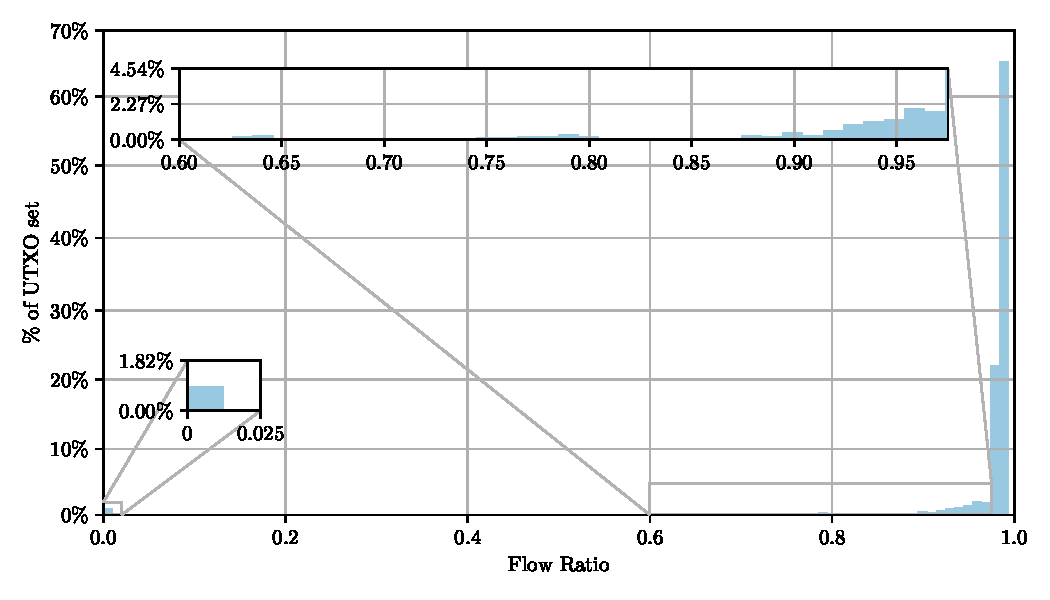
\includegraphics[width=0.8\textwidth]{Figures/utxo_hist2.pdf}
  \caption{The distribution of flow ratio for outputs in the URTO set.}
  \label{utxo-plot}
\end{figure}

\section{Results}
\label{scn:Results}


For our analysis, we used a snapshot of the Grin blockchain from March 17, 2020 containing 612,102 blocks.
As historical blocks are not available for download from the Grin P2P network, we were fortunate to obtain a PostgreSQL database containing the blockchain data from the administrator of the GrinExplorer website.
We used the community edition of the Neo4j graph database for the construction of the flow graph and flow upper bound calculations.
%The preprocessing of the blockchain data involved filtering out blocks in invalid (forked) side-chains.
%We also have taken care of same output commitments appearing more than once on the blockchain.


Figure \ref{ratio-plot} shows scatter plots of the flow ratio as a function of the block height, \textit{only for blocks with at least one RTO}. Note that the flow ratio corresponding to a block height is the flow ratio for all RTOs in the block at that height. 
We used a step size of 10 in the block height to reduce calculation time (which still took 13.5 hours). 
The subplots in the left column plot the flow ratio for three block height range of approximately 612,000. 
The subplots in the right column plot the flow ratio for the same block height ranges but with y-axis ranges 0.85 to 1, 0.9 to 1, and 0.95 to 1. 
The left column subplots show that while the flow ratio was initially small it had exceeded 0.9 for most blocks by block height 50,000. 
We found that 88\% of the blocks we considered had a flow ratio above 0.9. However, there were still block heights with small flow ratios even at heights larger than 100,000. 
For instance, about 6.6\% of the blocks we considered with heights larger than 100,000 had a flow ratio less than 0.5.
The column subplots on the right reveal a jagged structure in the scatter plots for flow ratios close to 1. While a precise explanation eludes us at this point, we suspect that the rising edges are due to the accumulation of coins by miners while the falling edges are due to the increase in the trivial upper bound in the flow ratio denominator.

%We refer to the ratio of upper bound computed using the graph approach and that of the trivial upper bound as \textit{flow ratio}.
%Figure \ref{ratio-plot} demonstrates that the flow ratio for transaction outputs in blocks climbs fast towards unity as the block height increases.
%% Note that we consider only transaction outputs in a block since the amounts in coinbase outputs are known trivially. 
%% The computed upper bound for blocks with height less than $25000$ are respectably lower than the trivial upper bound.
%For a mere $7\%$ of the blocks on the blockchain, the flow ratio is less than $0.5$,
%implying a significant difference between the computed and the trivial upper bounds. 
%The flow ratio for more than $87\%$ blocks is greater than $0.9$.
%% For the rest of the blocks, the difference between the computed and the trivial upper bound is not significant.
%This implies that the confidentiality of amounts hidden in the outputs in most blocks is preserved.
%Further, as the blockchain grows, the subgraphs for recent blocks naturally grow larger in terms of the donor nodes.
%This results in the flow ratio for most of the recent blocks inching towards unity. 
%
%An interesting find in the zoomed flow ratio plots in the lower axis of Figure \ref{ratio-plot} is that the flow ratio shows periodic jumps with respect to block height.
%A possible interpretation of this could be that near such block heights, there could be heavy density of incoming edges from coinbase outputs as well as from other blocks.
%The precise analysis for the reasons of such periodicity is an interesting direction of future research.
%% Graph analysis of Grin blockchain opens up many interesting avenues for research.

To get an idea of the current state of the Grin blockchain, we plot the distribution of flow ratio for only unspent regular transaction outputs (URTOs) in our snapshot in Figure \ref{utxo-plot}. We find that while 95\% of the 110,149 URTOs have a flow ratio greater than 0.9, about 0.8\% of them have a flow ratio less than 0.01. In terms of upper bounds, we found that 983 of the URTOs have an upper bound of 1800 grins. We conclude that while the flow upper bound does not violate the confidentiality of most of the URTOs, it can constrain the amounts in some URTOs to a narrow range.

As noted earlier, we used a step size of 10 in the block height while computing flow ratio for RTOs in blocks.
We did so for two reasons: (i) Computing flow upper bounds per block is a computationally heavy process as the block height increases,
(ii) The trend observed in flow ratio for step size 10 and step size 1 is similar.
For example, Figure \ref{continuity-plot} shows flow ratio for blocks in range $[39000, 41000]$.
The top subplot plots flow ratio for each block in the range $[39000, 41000]$ while the bottom subplot plots for blocks in steps of 10.
Clearly, the trend is very similar in both the subplots.

\begin{figure}[!h]
    \centering
    \includegraphics[width=0.7\textwidth]{Figures/continuity_vs_steps.png}
    \caption{The distribution of flow ratio for outputs in the URTO set.}
    \label{continuity-plot}
\end{figure}
  


%While we examine the upper bounds on amounts hidden in transaction outputs per block, it is crucial to explore the upper bounds of 
%the unspent transaction output (UTXO) set. In Figure \ref{utxo-plot}, we plot the fraction of the UTXO set versus the flow ratio.
%We observe that more than $83\%$ of the UTXOs possess a flow ratio greater than $0.97$. 
%On the contrary, just $1\%$ of the total UTXOs have a ratio less than $0.1$. 
%Here too, we consider only the unspent transaction outputs and not the unspent coinbase outputs. 

% \begin{figure}[!h]
%   \centering
%   \subfloat[Ratio vs Block height]{{\includegraphics[width=4.4cm]{continuity_vs_steps.pdf} }}
%   \subfloat[\% of UTXO set vs Ratio]{{\includegraphics[width=4.5cm]{utxo_hist1.pdf} }}
%   \caption{2 Figures side by side}%
%   \label{fig:example}%
% \end{figure}




\section{Conclusion}
In this chapter, we explore the question of whether the transaction graph in Grin violates the confidentiality of amounts hidden in the Pedersen commitments corresponding to regular transaction outputs. We find that the confidentiality for most outputs is preserved if the linkability information between inputs and outputs is ignored. As incorporating linkability information will lead to tighter upper bounds, it is a direction worthy of more investigation. The presence of regular transaction outputs with small upper bounds shows that the perfectly hiding property of Pedersen commitments in MimbleWimble-based cryptocurrencies should be taken with a grain of salt.  
We also intend to examine in future if similar analysis if possible for other cryptocurrency systems like Beam and Monero which use Pedersen Commitments.


%Analysing the Grin blockchain as a graph, we find upper bounds on the amounts hidden in the transaction outputs per block to comment on the confidentiality of amounts. 
%We conclude that the upper bounds on the amounts in the transaction outputs in more than $87\%$ of the blocks reveal negligible information above what is known trivially.
%Thus, our study backs up the claim of amount confidentiality in Grin outputs. 
% 
%In out study, we assume that the transactions in the Grin blocks are aggregated.
%It is possible to get information about individual transactions by listening to sufficient number of peer nodes since the transaction pool contains very few transactions.
%This would help establish significantly compact upper bounds on the amounts in outputs in disintegrated transactions.
%Such online analysis of the Grin blockchain is an exciting direction of future research.  
